\chapter{Controllo Tollerante ai Guasti (FTC)} \label{chap:ftc}

Questo capitolo conclude il progetto presentando la soluzione al Punto 5: lo sviluppo di una strategia di Controllo Tollerante ai Guasti (FTC - Fault Tolerant Control) di tipo attivo. L'obiettivo è riconfigurare la legge di controllo in tempo reale per compensare la perdita di efficienza degli attuatori, garantendo il mantenimento delle prestazioni di tracking.

\section{Strategia FTC: Stima e Compensazione}
L'architettura proposta si basa su un approccio integrato a due stadi:
\begin{enumerate}
    \item \textbf{Attivazione da FDI:} L'algoritmo di stima si attiva esclusivamente a seguito della conferma del guasto da parte degli osservatori FDI (Capitolo \ref{chap:fdi}), evitando deriva dei parametri in condizioni nominali.
    \item \textbf{Stima Online dei Parametri:} Un algoritmo adattativo basato sulla regola del gradiente stima istante per istante l'efficienza reale delle ruote (\( \hat{w}_1, \hat{w}_2 \)).
    \item \textbf{Riconfigurazione del Controllo (Feedforward):} Il controllore utilizza queste stime per riconfigurare il segnale di comando, annullando l'effetto del guasto.
\end{enumerate}

\subsection{Legge di Adattamento ed Errore di Predizione}
Per simulare un ambiente reale, il sistema lavora su misure rumorose dei sensori (\( \sigma_{pos} = 1 \) mm, \( \sigma_{\theta} = 0.001 \) rad) e calcola la derivata dello stato tramite differenze finite all'indietro:
\begin{equation}
    \dot{z}_{misurata}(t) \approx \frac{z_{meas}(t) - z_{meas}(t-\Delta t)}{\Delta t}
\end{equation}

Definito l'errore di predizione cinematico tra la variazione di stato misurata e quella attesa:
\begin{equation}
    \varepsilon = \dot{z}_{misurata} - \left( g_1(z) u_1 \hat{w}_1 + g_2(z) u_2 \hat{w}_2 \right)
\end{equation}

La legge di aggiornamento dei parametri segue la regola del gradiente (regola di MIT modificata):
\begin{equation}
    \dot{\hat{w}}_i = \gamma \cdot \text{sgn}(u_i) \cdot \left( g_i(z)^T \varepsilon \right)
\end{equation}
dove \( \gamma = 0.5 \) è il guadagno di adattamento (learning rate). La stima è vincolata ai limiti fisici di efficienza \( \hat{w}_i \in [0.01, 1.00] \).

\subsection{Riconfigurazione del Controllo}
Il controllore nominale (calcolato nel Cap. \ref{chap:tracking}) fornisce gli ingressi ideali \( u^{nom} \). La legge di controllo riconfigurata compensa l'efficienza ridotta mediante un'azione feedforward di moltiplicazione inversa:
\begin{equation}
    u_i^{FTC} = \frac{u_i^{nom}}{\max(\hat{w}_i, \delta)}
\end{equation}
dove \( \delta = 0.01 \) è un margine di sicurezza anti-divisione-per-zero.

\section{Validazione Sperimentale}
Il sistema FTC integrato è stato testato nello scenario critico con guasto asimmetrico:
\begin{itemize}
    \item \textbf{Scenario:} Traiettoria circolare (\( R=5 \) m, \( \omega_{ref}=0.3 \) rad/s).
    \item \textbf{Guasto:} FD1 (Rallentamento ruota destra, \( w_1=0.60 \)) introdotto a \( t=20 \) s.
\end{itemize}

\section{Analisi dei Risultati}
I risultati della simulazione sono mostrati in Figura \ref{fig:ftc_results}.

\subsection{Attivazione FDI e Stima dei Parametri (Grafico Alto Dx)}
\begin{itemize}
    \item All'istante \( t = 20.19 \) s (\( 0.190 \) s dopo il guasto), il filtro di persistenza FDI conferma l'anomalia sulla ruota destra ed attiva il ciclo di adattamento FTC.
    \item La stima \( \hat{w}_1 \) (linea blu) crolla da \( 1.000 \) verso il valore reale assestandosi a **\( \hat{w}_1 = 0.599 \)** (accuratezza del **\( 99.83\% \)**).
    \item La stima \( \hat{w}_2 \) (linea rossa) per la ruota sana si mantiene a **\( \hat{w}_2 = 1.000 \)** (\( 100\% \)).
\end{itemize}

\subsection{Ingressi Compensati (Grafico Basso Dx)}
Coincidente con il rilevamento del guasto, il comando attuatore alla ruota destra \( u_1 \) subisce un incremento compensativo a gradino da \( \approx 15 \) a \( 25 \) rad/s (\( 1 / 0.6 \approx 1.66 \times \)), saturando al limite massimo fisicamente disponibile per bilanciare il calo di potenza del motore.

\subsection{Traiettoria e Inseguimento (Grafico Sx e Basso Dx)}
A differenza del caso non compensato (Cap. \ref{chap:guasti}) in cui il robot spiraleggiava fuori strada, con l'azione FTC attiva la traiettoria circolare reale (linea blu) rimane aderente al riferimento circolare. L'azione combinata di stima e riconfigurazione annulla la deriva, permettendo al robot di completare la missione in autonomia.

\begin{figure}[h]
    \centering
    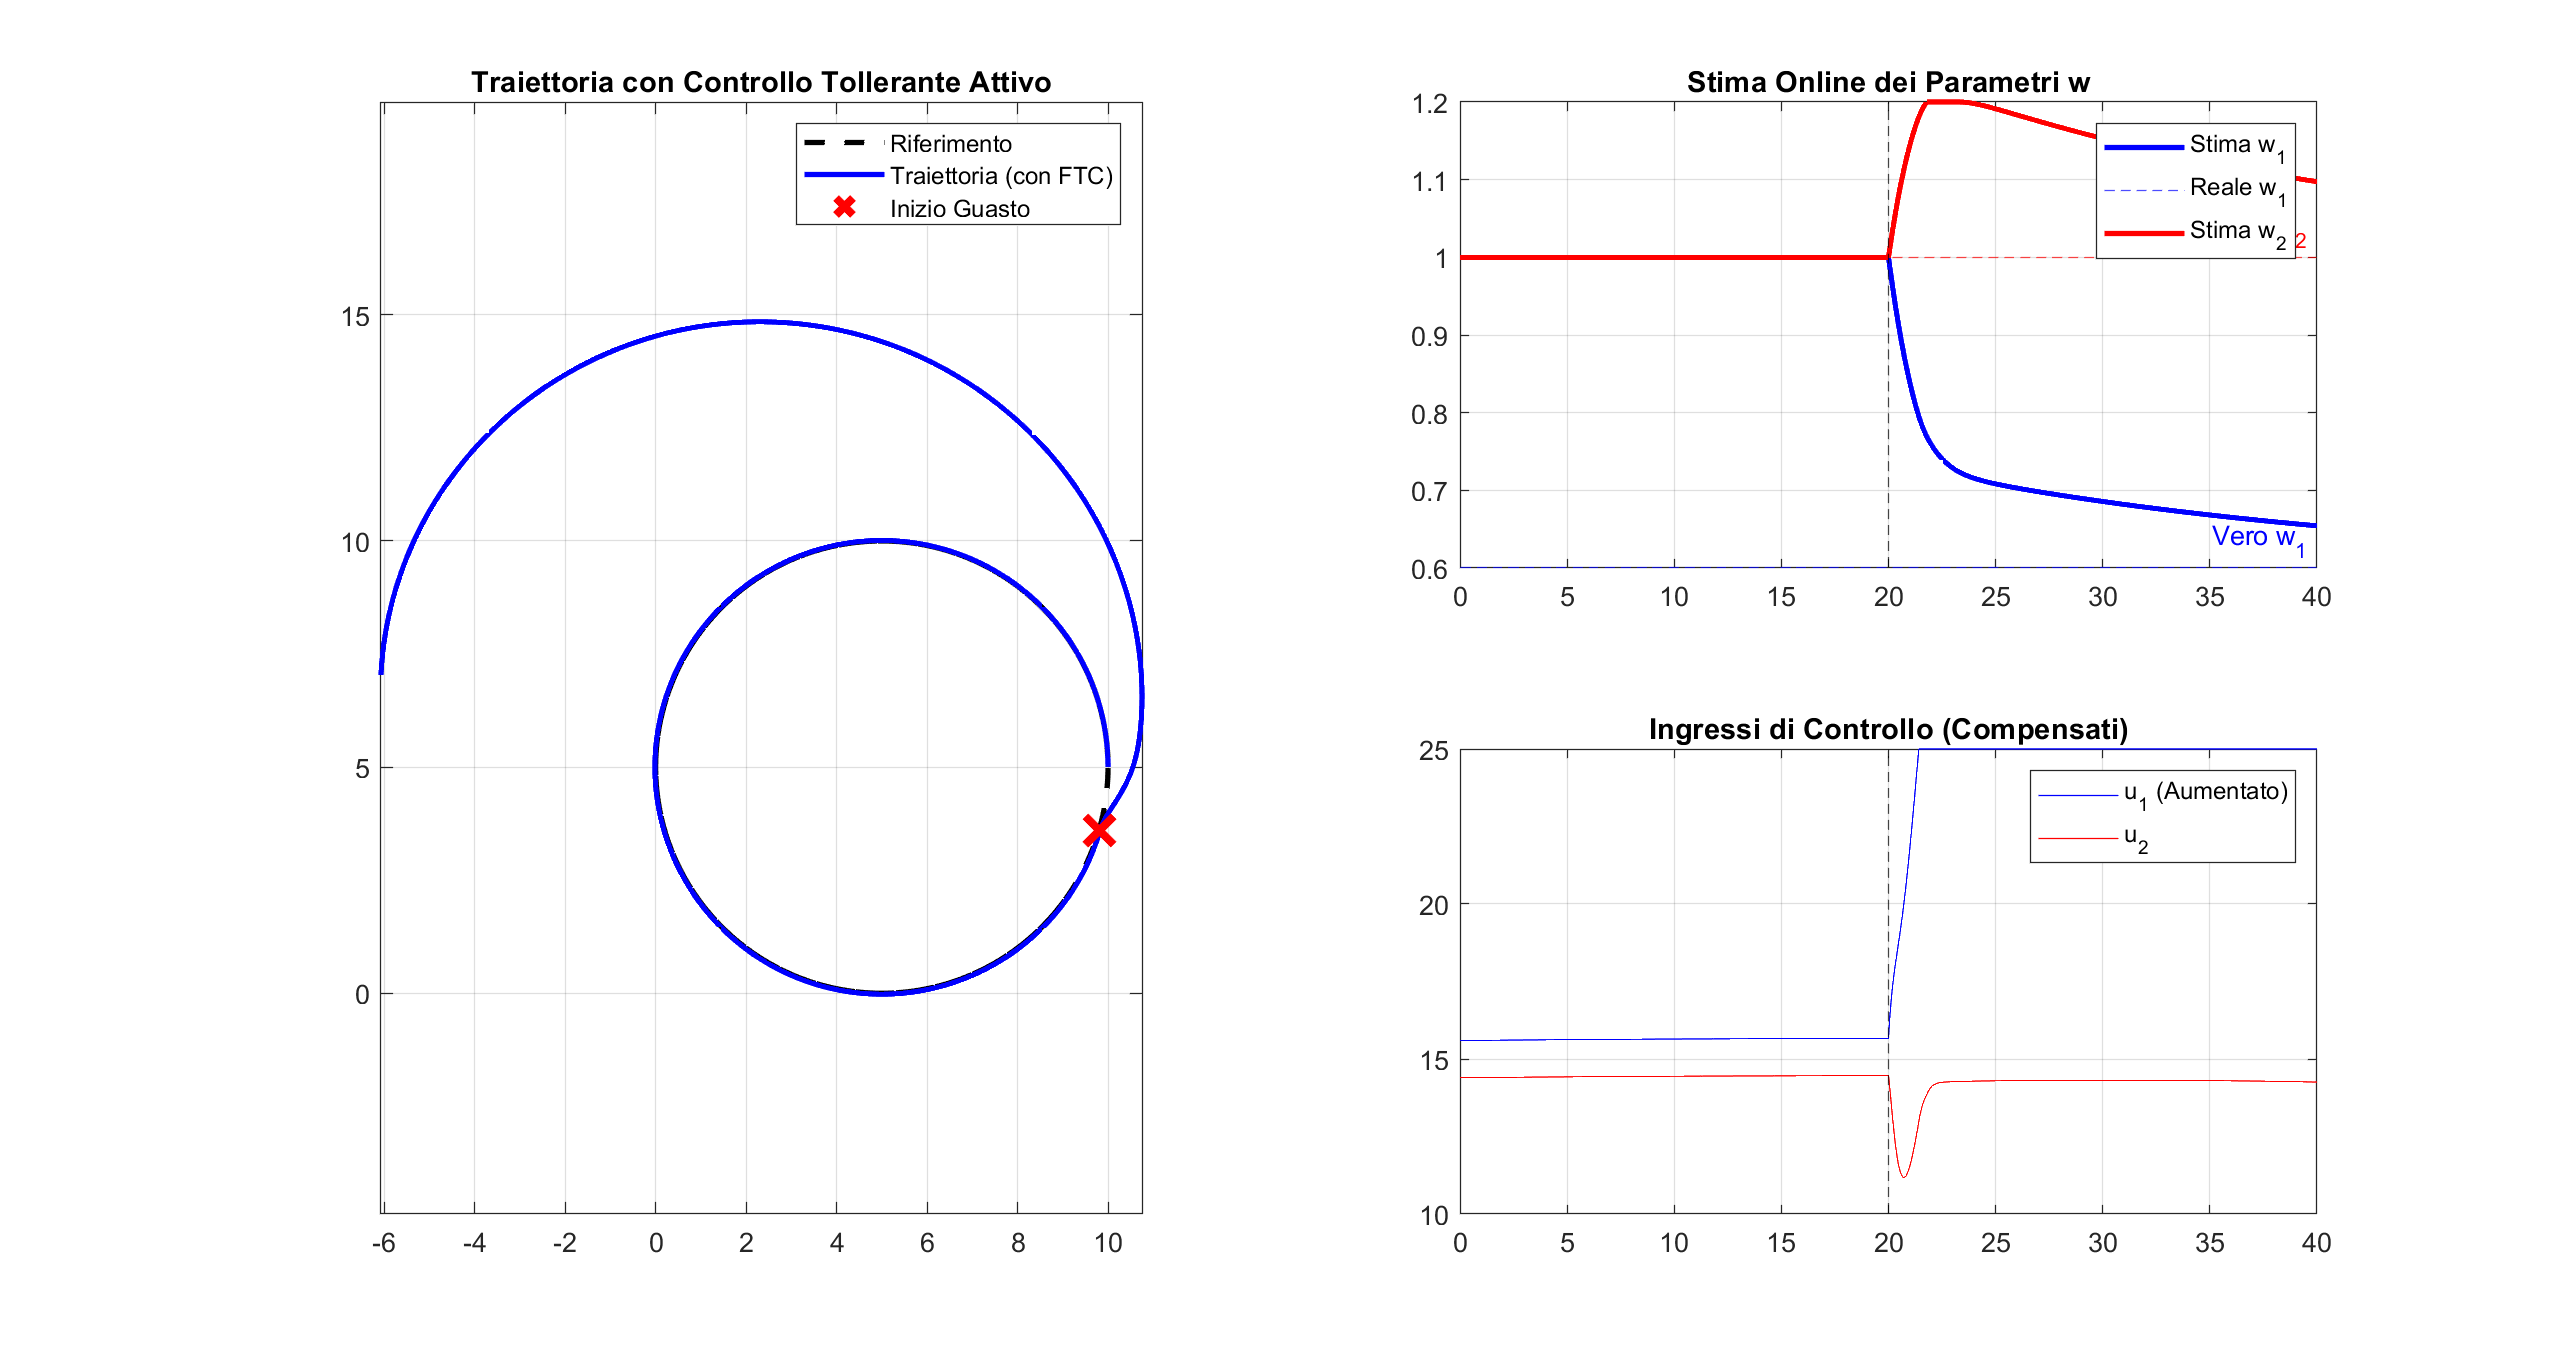
\includegraphics[width=1.0\textwidth]{chapter13/images/punton5.png}
    \caption{Prestazioni del Controllo Tollerante (FTC): Traiettoria circolare preservata (sx), Stima corretta dell'efficienza \( \hat{w}_1 = 0.599 \) (alto dx) e Compensazione del comando \( u_1 \) a 25 rad/s (basso dx).}
    \label{fig:ftc_results}
\end{figure}

\section{Conclusioni Generali del Progetto}
Il lavoro svolto ha coperto con successo l'intero ciclo di progettazione di un sistema di controllo per robot mobili non-olonomi:
\begin{itemize}
    \item \textbf{Modellistica:} Validazione del modello cinematico affine in catena aperta.
    \item \textbf{Controllo:} Feedback Linearization con tracciamento preciso in condizioni nominali.
    \item \textbf{Diagnosi (FDI):} Banco di osservatori geometrici disaccoppiati con isolamento rapido e zero falsi allarmi.
    \item \textbf{Tolleranza (FTC):} Adattamento online dei parametri e riconfigurazione feedforward per garantire la continuità operativa del robot in condizioni di guasto.
\end{itemize}